\subsection{Deterministic Policy Gradient Algorithms}
\label{sec:survey:DPG}
앞서 살펴본 DQN과 같은 방법은 value function을 학습하는 방식이기 때문에 만약 value가 살짝 바뀌어도 policy가 같이 변하여 학습 과정이 불안정하게 되고 수렴이 불안정해지는 단점이 있다. 
따라서 policy 자체를 예측을 하면 되지 않을까라는 개념으로 탄생한 것이 policy gradient 알고리즘이다. 

policy gradient 알고리즘은 expected reward를 policy의 파라미터에 대한 함수로 모델링하고 이 reward를 최대화하는 policy를 gradient ascent 기법을 사용해서 찾는 기법이다.
해당 기법은 policy의 변화를 통해 더 나은 policy를 찾아가는 방식으로 구성되어 있다. 
최적의 policy는 stochastic한 성질을 가지는 경우가 많기 때문에 stochastic policy gradient 방식을 선호하였는데 해당 논문을 통해 deterministic policy gradient가 high-dimensional task에서 보다 빠르게 동작한다는 것을 증명하였다. 

해당 논문에서는 octopus arm 실험을 통해 성능을 측정하였는데 해당 실험을 사용한 이유는 high dimensional task에서의 성능을 확인하기 위함이다 (Figure~\ref{fig:dueling_network} 참조).
해당 실험에서 목표는 6 개의 구획으로 구성된 다리를 움직여 오렌지 색상의 음식을 검은색 입으로 전달하여 보상을 얻는 것이다.
환경에서는 50 개의 continuous 한 state가 존재하며 각 구획에는 회전 및 이동할 수 있는 muscle이 존재해 한 구획당 총 20 가지의 동작이 가능하다. 
이러한 실험에서 높은 성능을 보였고 high dimensional 한 task에서는 deterministic policy gradient 알고리즘이 stochastic의 경우보다 성능이 좋다는 것을 확인하였다.

\begin{figure}[h]
\begin{center}
\begin{tabular}{c}
     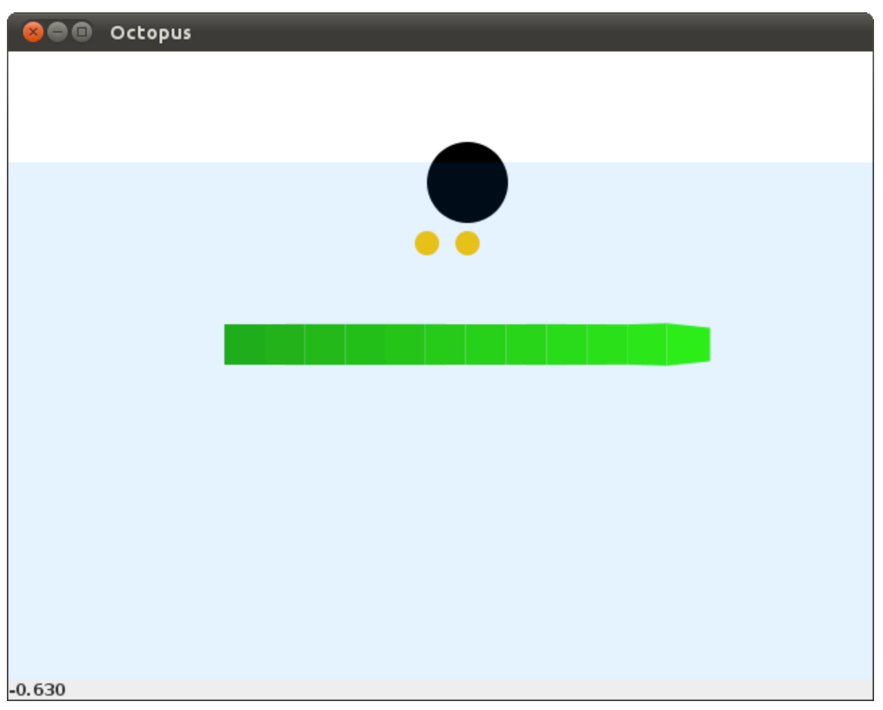
\includegraphics[width=0.45\textwidth]{FIG/OctopusArm.png} \\
\end{tabular}
\caption{
	Octopus Arm Environment.
}
\label{fig:octopus_arm}
\end{center}
\end{figure}

policy gradient 알고리즘은 continuous 한 action space 상황에서 자주 사용되는데 본 프로젝트에서 실험하는 슈퍼 마리오 브라더스는 discrete 한 action space 상황이기 때문에 deterministic policy gradient 알고리즘을 바로 적용할 수는 없다. 
그러나 해당 논문을 통해 우리 모델의 성능을 높이기 위해 policy gradient를 적용한다는 아이디어를 참고할 수 있기에 해당 논문을 서베이 목록에 추가하였다.
